%% ============================================================
%%  CloudRAG: A Reproducible Benchmark and Hybrid Retrieval
%%  Pipeline for Multi-Cloud Technical Documentation
%%  LACCI 2026  --  IEEE Conference Paper (max 6 pages)
%% ============================================================
\documentclass[conference]{IEEEtran}
\IEEEoverridecommandlockouts
% ---- Core packages (IEEE approved) ----
\usepackage{cite}
\usepackage{amsmath,amssymb,amsfonts}
\usepackage{algorithmic}
\usepackage{graphicx}
\graphicspath{{figures/}}
\usepackage{textcomp}
\usepackage{xcolor}
\usepackage{booktabs}
\usepackage{url}
\usepackage[hidelinks]{hyperref}
% BibTeX helper (from IEEE template)
\def\BibTeX{{\rm B\kern-.05em{\sc i\kern-.025em b}\kern-.08em
    T\kern-.1667em\lower.7ex\hbox{E}\kern-.125emX}}

\begin{document}

% ============================================================
%  TITLE + AUTHORS
% ============================================================
\title{CloudRAG: A Reproducible Benchmark and Hybrid Retrieval Pipeline for Multi-Cloud Technical Documentation%
\thanks{This research was conducted as part of the undergraduate thesis work of the first author at Universidad de Lima, Peru.}
}

% TODO: CONFIRM WITH LEWIS IF HE CO-AUTHORS.
% If he declines, remove the second \IEEEauthorblock block and move him to Acknowledgments.
\author{
\IEEEauthorblockN{Enzo F. Ordo\~{n}ez Flores}
\IEEEauthorblockA{\textit{Facultad de Ingenier\'{i}a de Sistemas} \\
\textit{Universidad de Lima}\\
Lima, Peru \\
20221789@aloe.ulima.edu.pe}
\and
\IEEEauthorblockN{Lewis Fuentes Winston}
\IEEEauthorblockA{\textit{Facultad de Ingenier\'{i}a de Sistemas} \\
\textit{Universidad de Lima}\\
Lima, Peru \\
lfuentes@ulima.edu.pe \% TODO: VERIFY REAL EMAIL
}
}

\maketitle

% ============================================================
%  ABSTRACT
% ============================================================
\begin{abstract}
Retrieval-Augmented Generation (RAG) systems are a promising approach to
ground Large Language Models on specialized technical corpora, yet retrieval
quality over multi-vendor cloud documentation remains under-studied. We
present CloudRAG, a reproducible benchmark and a hybrid retrieval pipeline
for technical documentation spanning Amazon Web Services, Microsoft Azure,
and Google Cloud Platform. CloudRAG combines sparse lexical retrieval (BM25)
with dense semantic retrieval (BGE-large-en-v1.5) fused through Reciprocal
Rank Fusion, a cross-encoder reranking stage (ms-marco-MiniLM-L-12-v2), a
cross-cloud terminology normalization module, and a Natural Language
Inference based faithfulness filter. On a 200-query expert-curated test
set, the hybrid pipeline achieves P@1 = 0.930, MRR = 0.942, and
NDCG@5 = 0.736, outperforming BM25 (P@1 = 0.785) and dense retrieval alone
(P@1 = 0.860) with statistical significance (Wilcoxon signed-rank test,
p < 0.0001; Cohen's d = 0.626). Cross-cloud terminology normalization
contributes a 16.8 percent gain in answer faithfulness over an unnormalized
baseline. We release the dataset, code, evaluation harness, and Docker
artifacts to enable direct replication.
\end{abstract}

\begin{IEEEkeywords}
Retrieval-Augmented Generation, Hybrid Retrieval, Reciprocal Rank Fusion, Cross-Encoder Reranking, Cloud Documentation, Natural Language Inference, Hallucination Detection.
\end{IEEEkeywords}

% ============================================================
%  I. INTRODUCTION
% ============================================================
\section{Introduction}
\label{sec:intro}

% --- TODO: final prose. Current content = structured placeholders. ---
Large Language Models (LLMs) produce fluent text but hallucinate when queried
about specialized technical knowledge under-represented in their
pre-training corpora~\cite{lewis2020rag,ji2023hallucination}.
Retrieval-Augmented Generation (RAG) mitigates this by grounding generation
in an external corpus retrieved at inference time~\cite{lewis2020rag,gao2024ragsurvey}.

\textcolor{blue}{[PLACEHOLDER: Motivate cloud documentation specifically. (a) Multi-cloud is the enterprise norm; (b) documentation evolves weekly so LLM knowledge cutoffs are a hard constraint; (c) cross-cloud terminology drift (VPC $\leftrightarrow$ Virtual Network $\leftrightarrow$ VPC Network) breaks naive retrieval.]}

\textcolor{blue}{[PLACEHOLDER: State the gap. Existing RAG benchmarks (KILT, Natural Questions, MS MARCO) cover open-domain QA, not technical cloud documentation. Recent surveys and benchmarks~\cite{yu2024ragsurvey,gan2025ragevaluation,wang2025corbrag} do not evaluate cross-cloud terminology normalization.]}

Our contributions are:
\begin{itemize}
  \item A reproducible multi-cloud QA benchmark covering AWS, Azure, and GCP (200 expert queries with normalized gold evidence, plus 30 additional cross-cloud queries used in the normalization ablation).
  \item A cross-cloud terminology normalization module operating at both index and query time.
  \item A systematic ablation isolating the contribution of BM25, dense retrieval, RRF fusion, cross-encoder reranking, and NLI-based faithfulness filtering.
  \item An empirical trade-off study across three open-weight LLMs (Llama 3.1 8B, Mistral 7B, Qwen 2.5 7B) deployed locally via Ollama.
  \item An open-source reference implementation (code, data, Docker) for one-command replication.
\end{itemize}

\textcolor{blue}{[PLACEHOLDER: Close with roadmap. Section~\ref{sec:related} surveys related work; Section~\ref{sec:method} presents methodology; Section~\ref{sec:setup} the experimental setup; Section~\ref{sec:results} results; Section~\ref{sec:discussion} discussion; Section~\ref{sec:conclusion} conclusions.]}

% ============================================================
%  II. RELATED WORK
% ============================================================
\section{Related Work}
\label{sec:related}

\subsection{Sparse and Dense Retrieval}
\textcolor{blue}{[PLACEHOLDER: BM25~\cite{robertson2009bm25} remains a hard baseline; dense retrieval advanced with DPR~\cite{karpukhin2020dpr} and ColBERT's late interaction~\cite{khattab2020colbert}; modern encoders such as BGE~\cite{xiao2023bge} and efficient ANN indexing with FAISS~\cite{johnson2019faiss}.]}

\subsection{Hybrid Retrieval and Fusion}
\textcolor{blue}{[PLACEHOLDER: RRF~\cite{cormack2009rrf} is the canonical fusion method. Recent hybrid RAG evidence: Blended RAG~\cite{sawarkar2024blendedrag}, domain medical~\cite{aljohani2026hybrid}, performance-cost trade-offs~\cite{kartiyanta2025costeffective}.]}

\subsection{RAG Systems and Evaluation}
\textcolor{blue}{[PLACEHOLDER: RAG surveys~\cite{gao2024ragsurvey,yu2024ragsurvey}; failure analysis~\cite{barnett2024sevenfailure}; benchmarking~\cite{wang2025corbrag,gan2025ragevaluation,krishna2024factfetchreason}; four-module synergy~\cite{shi2024fourmodule}; chunking strategies~\cite{peng2025latesplit,jadon2025domainspecific}.]}

\subsection{Domain-Specific and Technical RAG}
\textcolor{blue}{[PLACEHOLDER: Technical PDFs~\cite{rahman2025techpdfs}; industrial semantic search with SHAP~\cite{mahr2025shap}; Azure-specific~\cite{mahmood2025azureiq}; digital twins Industry 4.0~\cite{xia2024digitaltwins}; precision/interpretability~\cite{hindi2025precision}. Position the gap: none address cross-cloud terminology normalization.]}

\subsection{Hallucination Detection}
\textcolor{blue}{[PLACEHOLDER: Hallucination taxonomy~\cite{ji2023hallucination}; NLI as faithfulness proxy~\cite{honovich2022true}. Motivate our DeBERTa-based NLI filter.]}

% ============================================================
%  III. METHODOLOGY
% ============================================================
\section{Methodology}
\label{sec:method}

\subsection{Pipeline Overview}
\textcolor{blue}{[PLACEHOLDER: Insert Fig.~\ref{fig:pipeline} (fig\_end\_to\_end.png). Describe 5 stages: (1) ingestion + normalization, (2) hybrid retrieval BM25+dense, (3) RRF fusion, (4) cross-encoder reranking, (5) generation + NLI faithfulness filter.]}

\begin{figure}[htbp]
\centerline{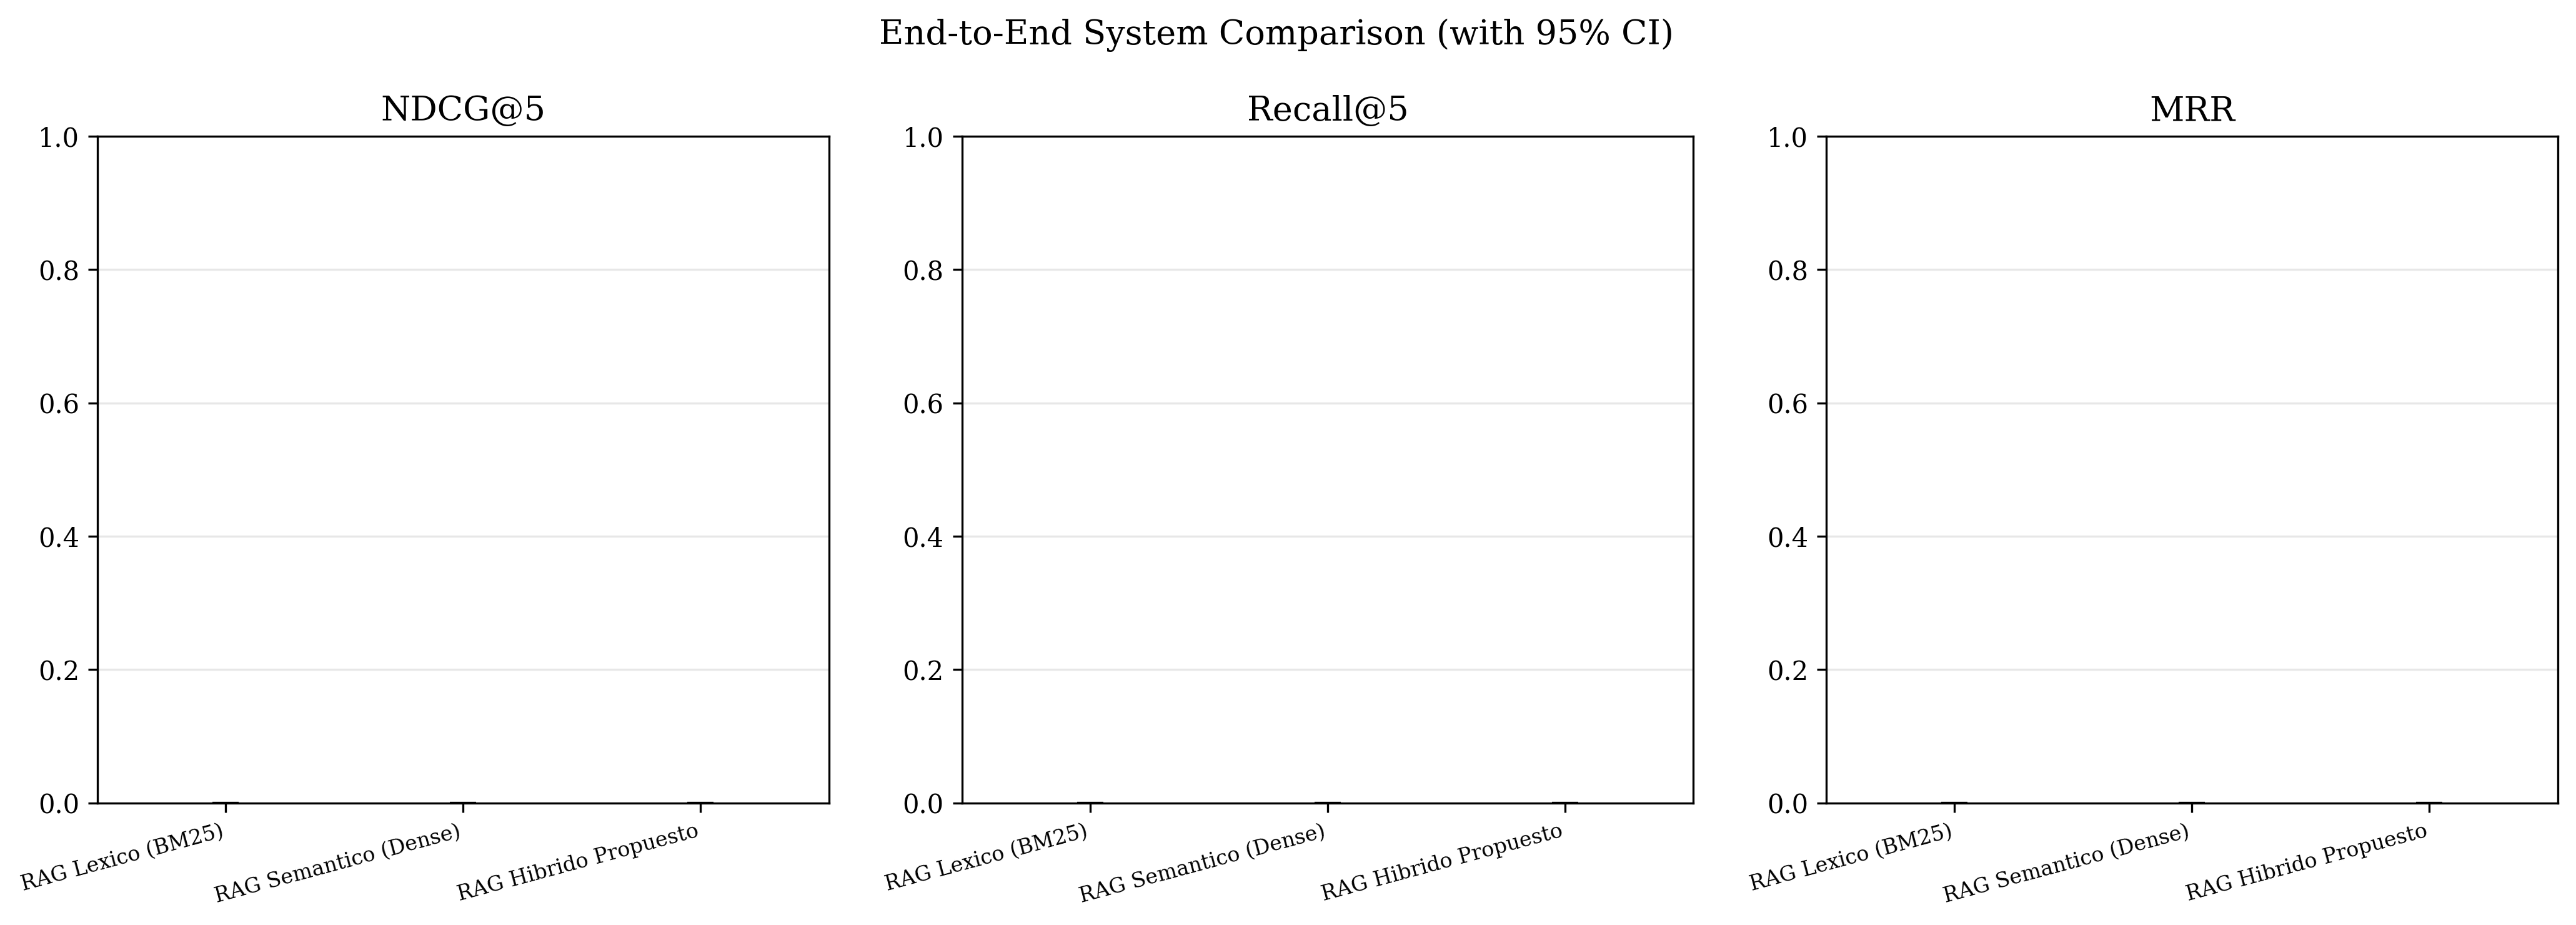
\includegraphics[width=\columnwidth]{fig_end_to_end.png}}
\caption{CloudRAG end-to-end pipeline.}
\label{fig:pipeline}
\end{figure}

\subsection{Corpus Construction and Preprocessing}
\textcolor{blue}{[PLACEHOLDER: Data sources: official AWS, Azure, GCP documentation. Crawler spec, deduplication, language filter. Corpus size, token counts, per-provider distribution. Crawl timestamp for reproducibility.]}

\subsection{Cross-Cloud Terminology Normalization}
\textcolor{blue}{[PLACEHOLDER: Curated alias table (e.g., \{VPC, Virtual Network, VPC Network\} $\to$ canonical token). Applied symmetrically at ingest and query time. Include Table of representative mappings.]}

\subsection{Chunking Strategy}
\textcolor{blue}{[PLACEHOLDER: Adaptive 500-token chunks respecting section boundaries, code blocks, and tables; compare against fixed-size. Cite~\cite{mahmood2025azureiq,mahr2025shap,rahman2025techpdfs}.]}

\subsection{Retrieval Components}
\textcolor{blue}{[PLACEHOLDER: BM25 parameters (k1, b). Dense: BGE-large-en-v1.5 (1024-dim), FAISS IVF-PQ index. RRF constant $k=60$. Top-$k$ per retriever. Cross-encoder reranker: ms-marco-MiniLM-L-12-v2.]}

\subsection{Generation and Faithfulness Filtering}
\textcolor{blue}{[PLACEHOLDER: Three local LLMs via Ollama (Llama 3.1 8B-instruct, Mistral 7B-instruct, Qwen 2.5 7B-instruct). Prompt template in Appendix. NLI filter applied claim-wise against retrieved evidence; threshold selection procedure.]}

% ============================================================
%  IV. EXPERIMENTAL SETUP
% ============================================================
\section{Experimental Setup}
\label{sec:setup}

\subsection{Benchmark}
\textcolor{blue}{[PLACEHOLDER: 200 expert-curated queries across AWS/Azure/GCP (exp1-6, exp8, exp8b), plus 30 additional cross-cloud queries used only in exp7. Query-type distribution (config / troubleshooting / conceptual / cross-cloud mapping). Gold evidence: document + span. Annotation protocol.]}

\subsection{Metrics}
\textcolor{blue}{[PLACEHOLDER: Retrieval: P@1, P@5, Recall@5, MRR, NDCG@5. Generation: faithfulness (NLI), answer accuracy (exact / LLM-as-judge). Efficiency: latency p50/p95, tokens.]}

\subsection{Statistical Protocol}
\textcolor{blue}{[PLACEHOLDER: Wilcoxon signed-rank over per-query deltas. Cohen's d for effect size. Bootstrap CIs (10{,}000 resamples).]}

\subsection{Implementation and Reproducibility}
\textcolor{blue}{[PLACEHOLDER: Hardware (CPU/GPU/RAM). Software: Python 3.11, sentence-transformers, faiss-cpu, Ollama. Docker image + Zenodo DOI + GitHub URL. Fixed random seeds.]}

% ============================================================
%  V. RESULTS
% ============================================================
\section{Results}
\label{sec:results}

\subsection{Retrieval Quality}
\textcolor{blue}{[PLACEHOLDER: Insert Table of retrieval metrics (from table\_retrieval\_metrics.tex). Insert Fig.~\ref{fig:retrieval} (fig\_retrieval\_comparison.png).]}

\begin{figure}[htbp]
\centerline{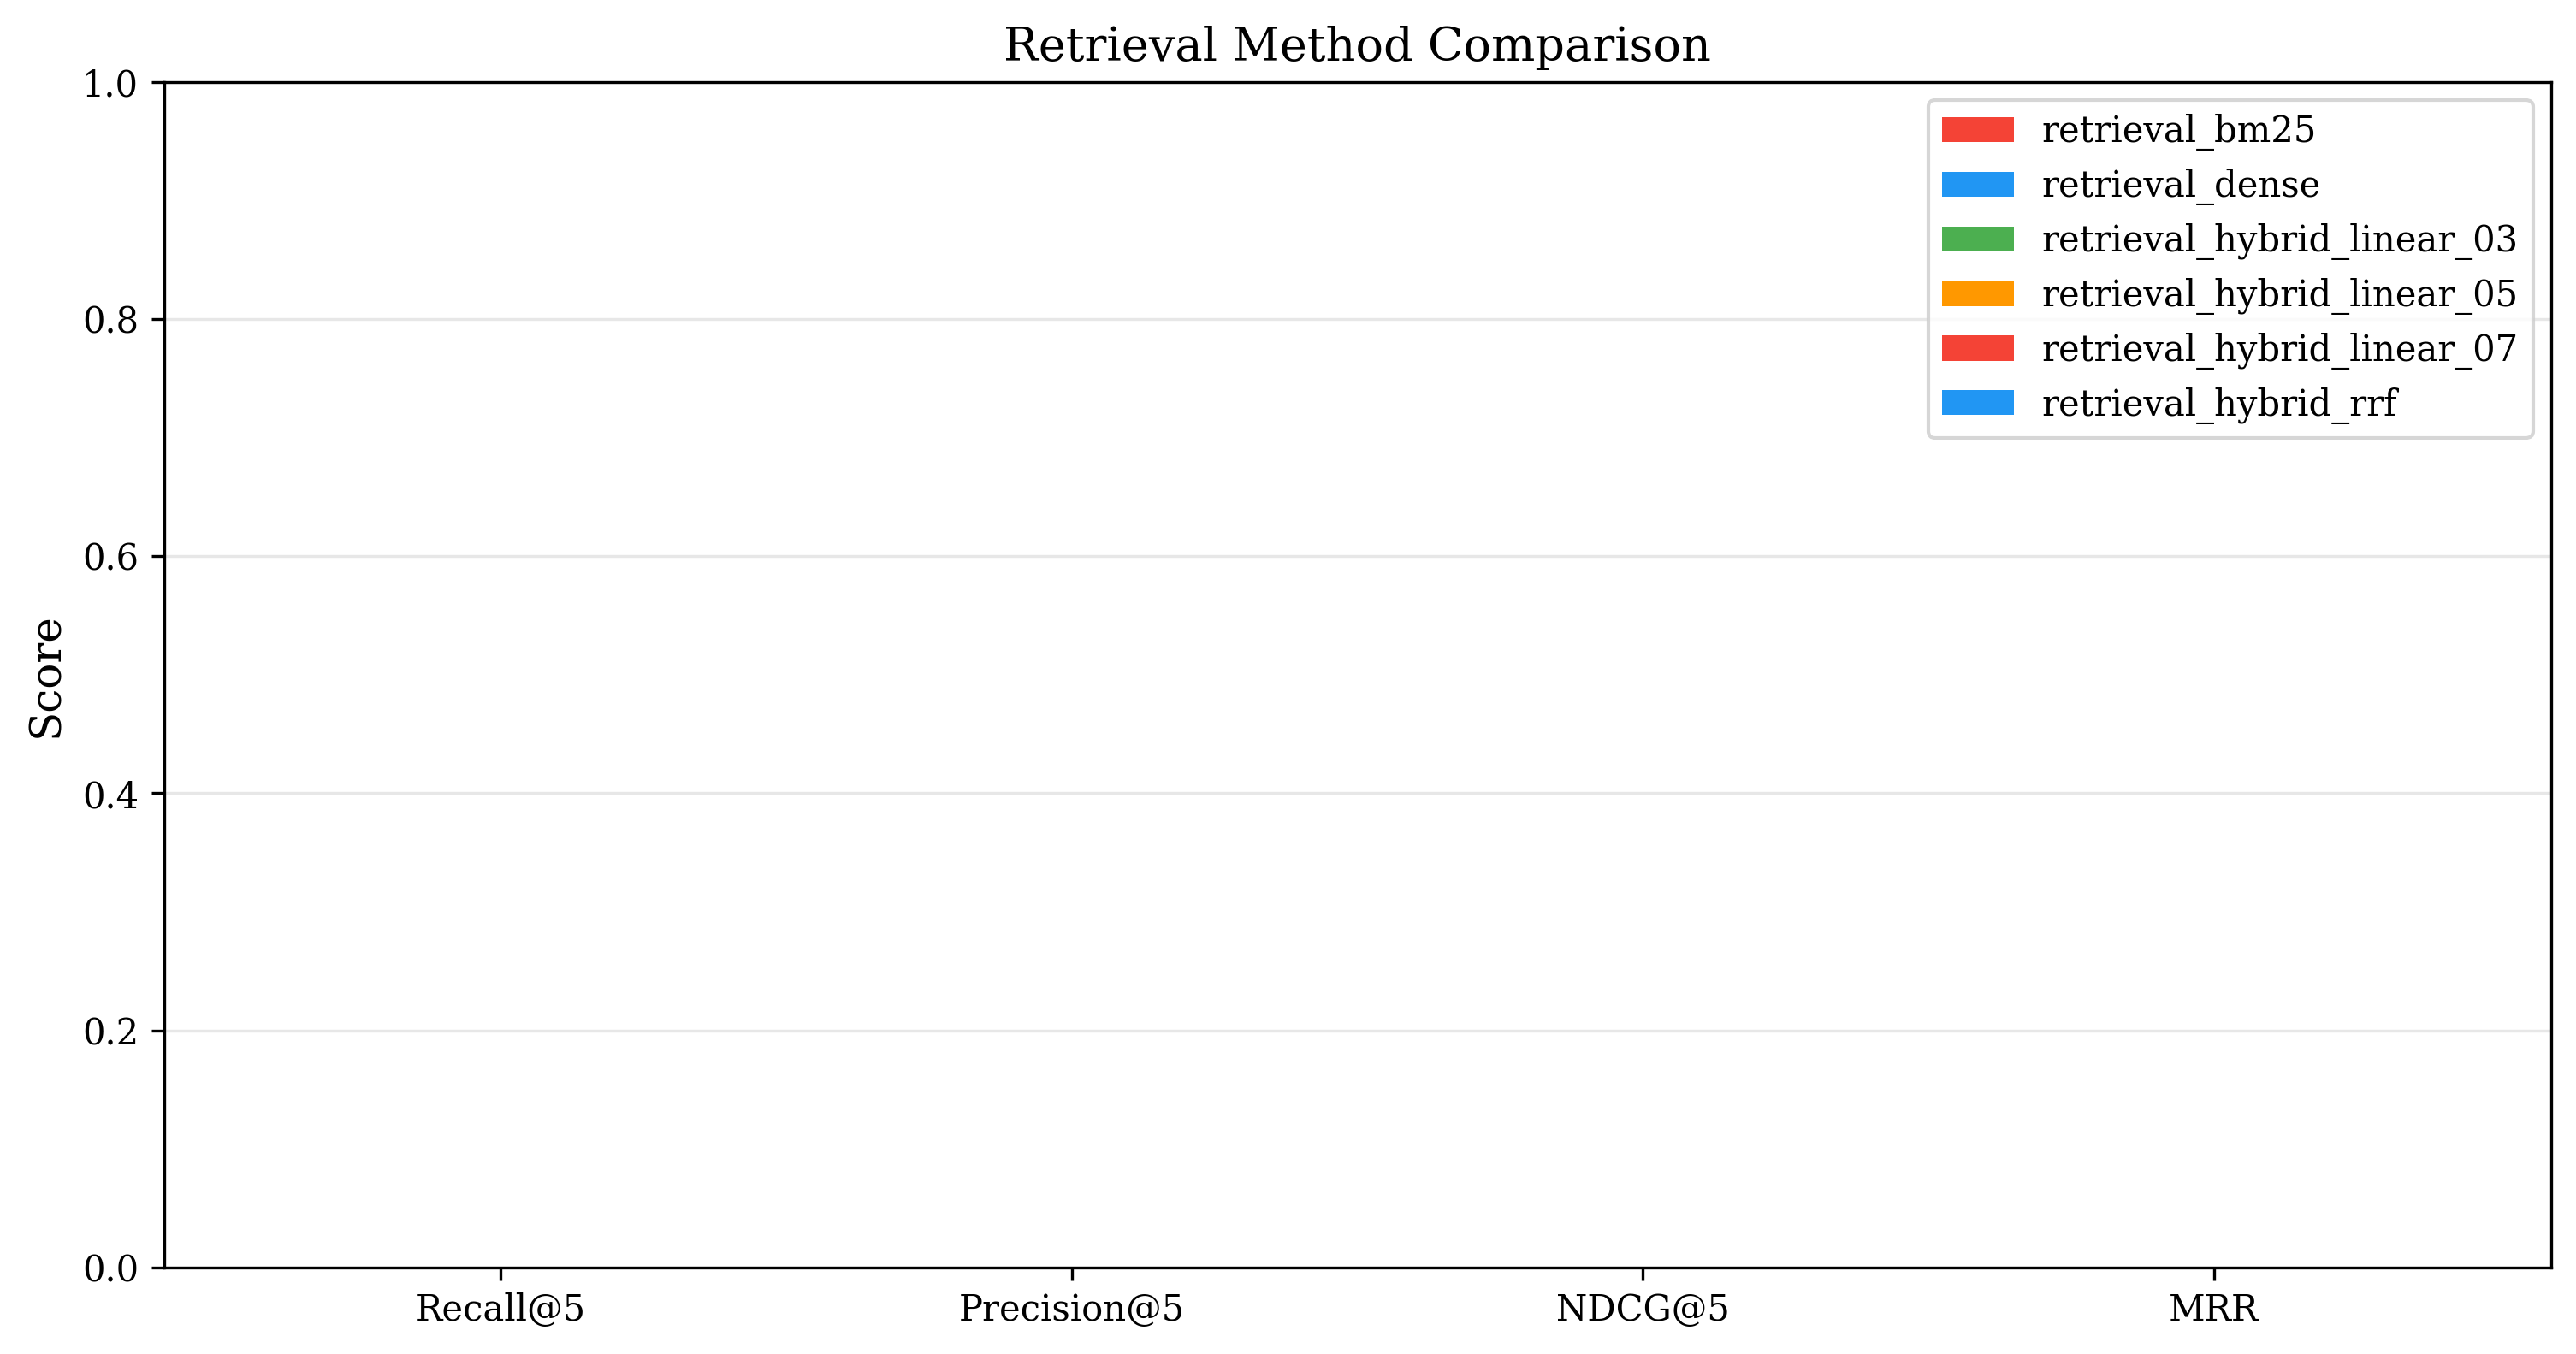
\includegraphics[width=\columnwidth]{fig_retrieval_comparison.png}}
\caption{Retrieval quality: BM25 vs.\ Dense vs.\ Hybrid vs.\ Hybrid+Reranker.}
\label{fig:retrieval}
\end{figure}

\subsection{Ablation Study}
\textcolor{blue}{[PLACEHOLDER: Insert Fig.~\ref{fig:ablation} (fig\_ablation\_waterfall.png). Drop each component one at a time; report $\Delta$NDCG@5 and $\Delta$Faithfulness.]}

\begin{figure}[htbp]
\centerline{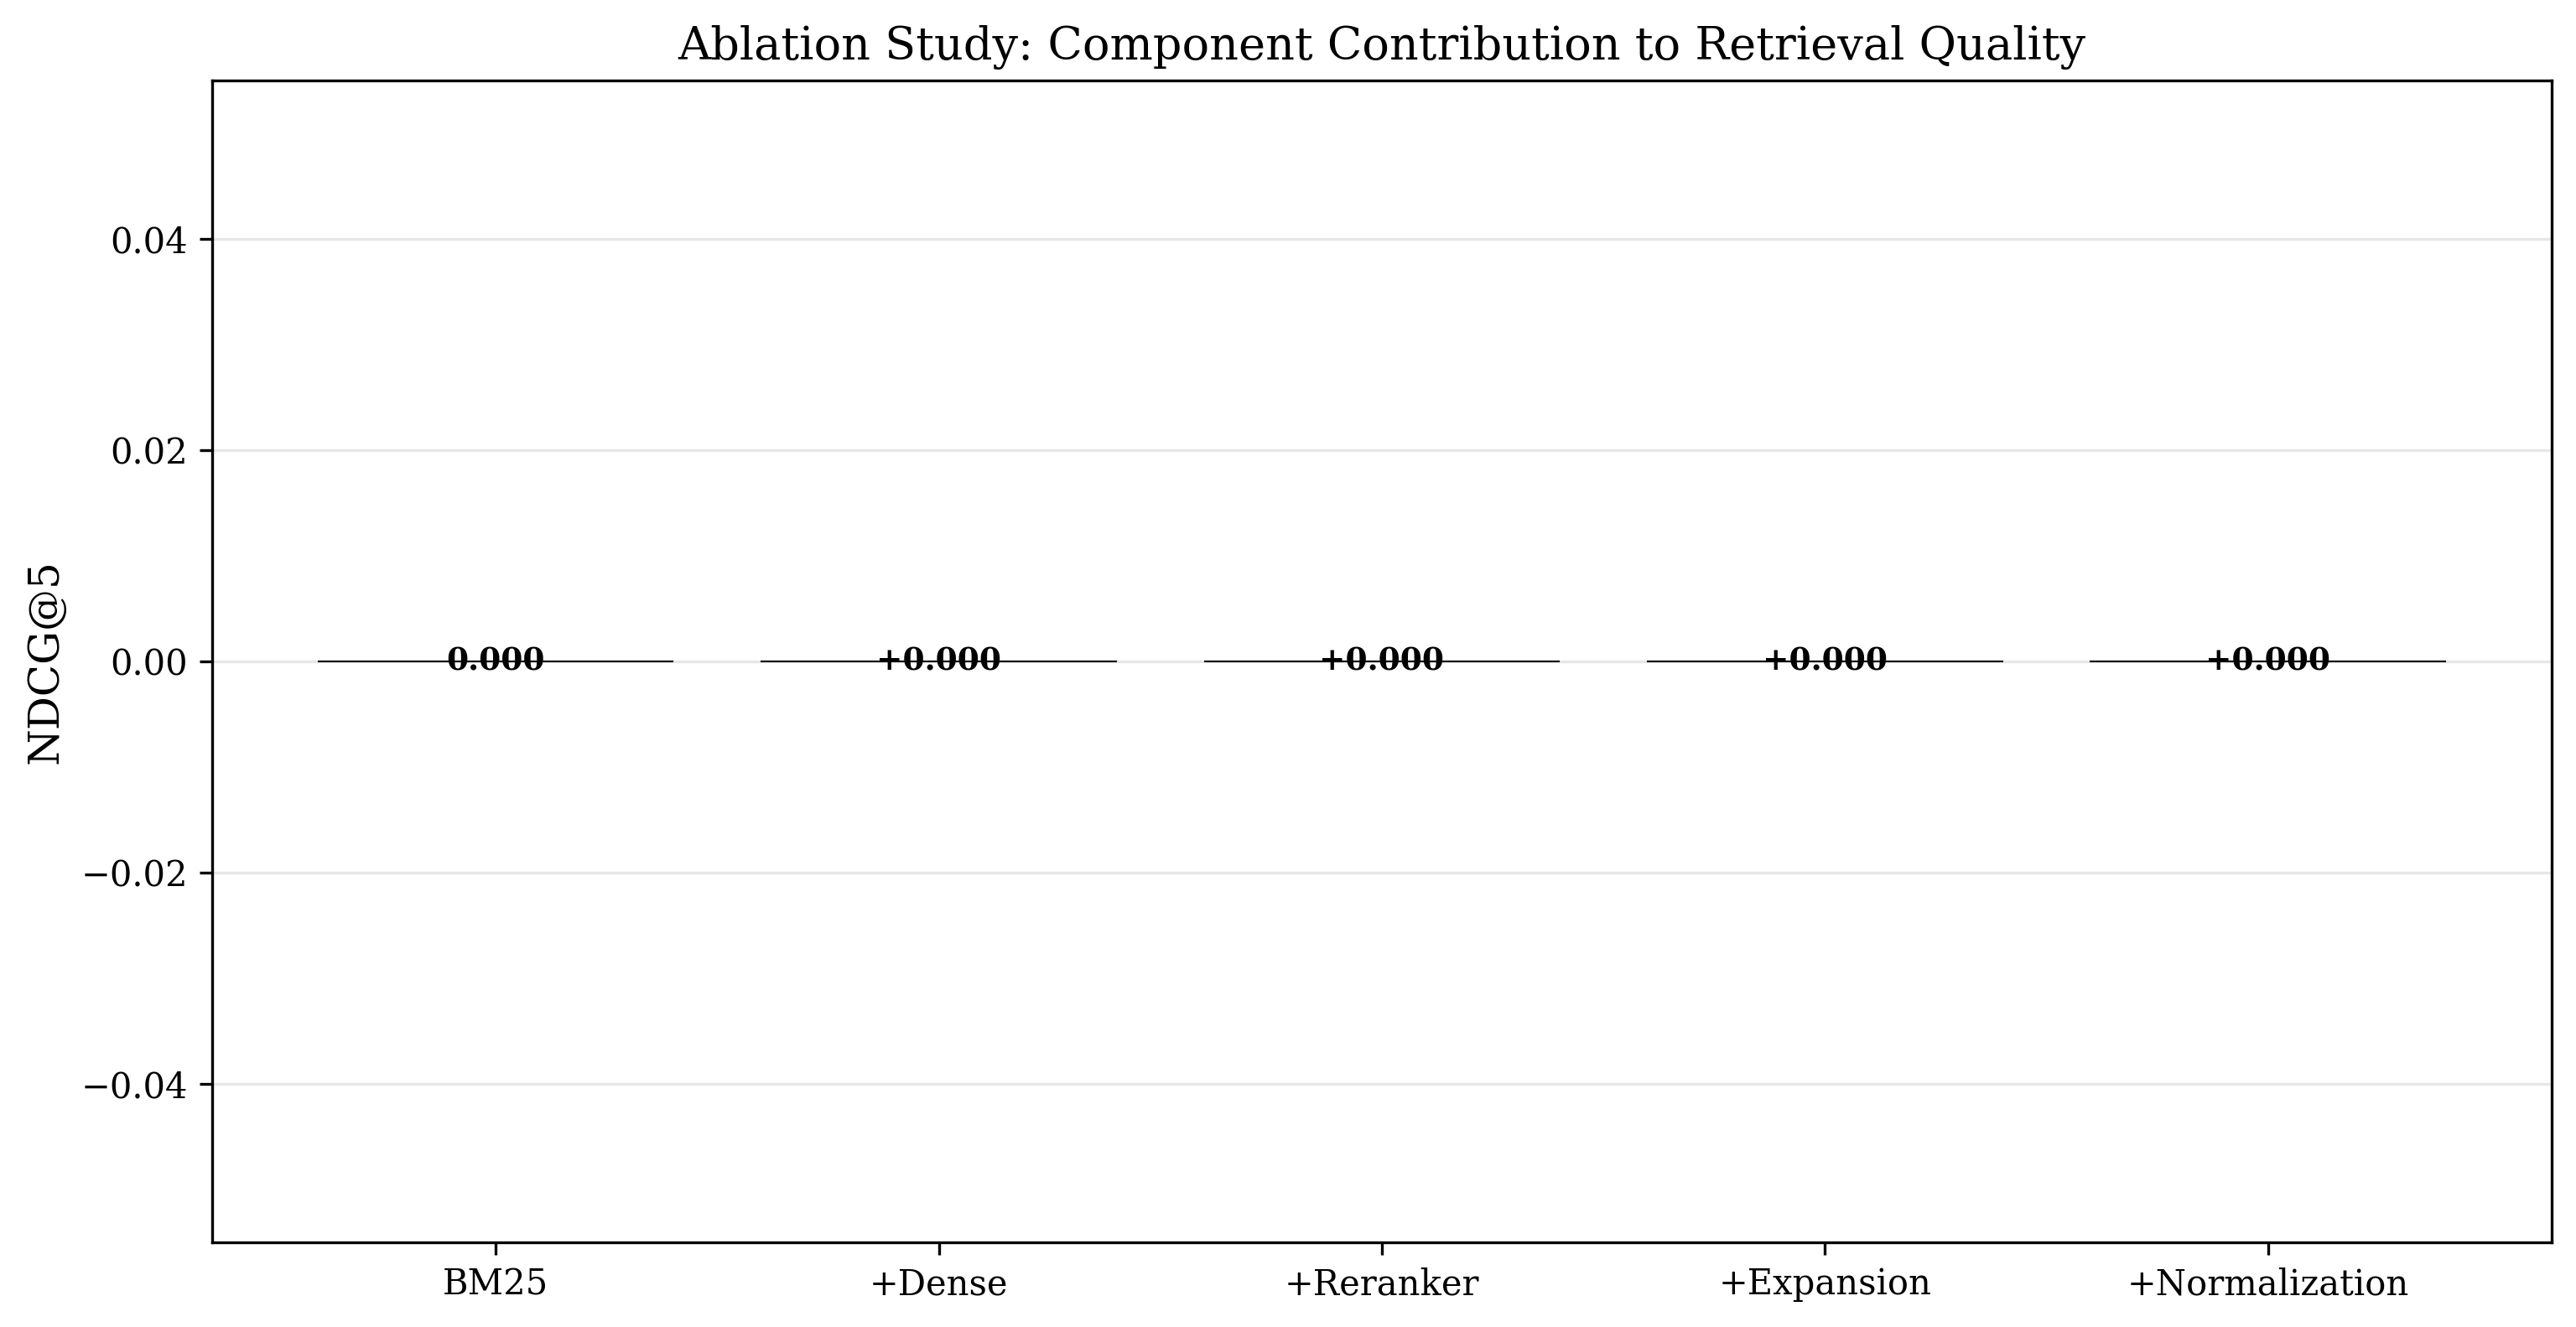
\includegraphics[width=\columnwidth]{fig_ablation_waterfall.png}}
\caption{Ablation waterfall of pipeline components.}
\label{fig:ablation}
\end{figure}

\subsection{Cross-Cloud Normalization Impact}
\textcolor{blue}{[PLACEHOLDER: Insert Fig.~\ref{fig:crosscloud} (fig\_cross\_cloud\_improvement.png). Report +16.8\% faithfulness gain.]}

\begin{figure}[htbp]
\centerline{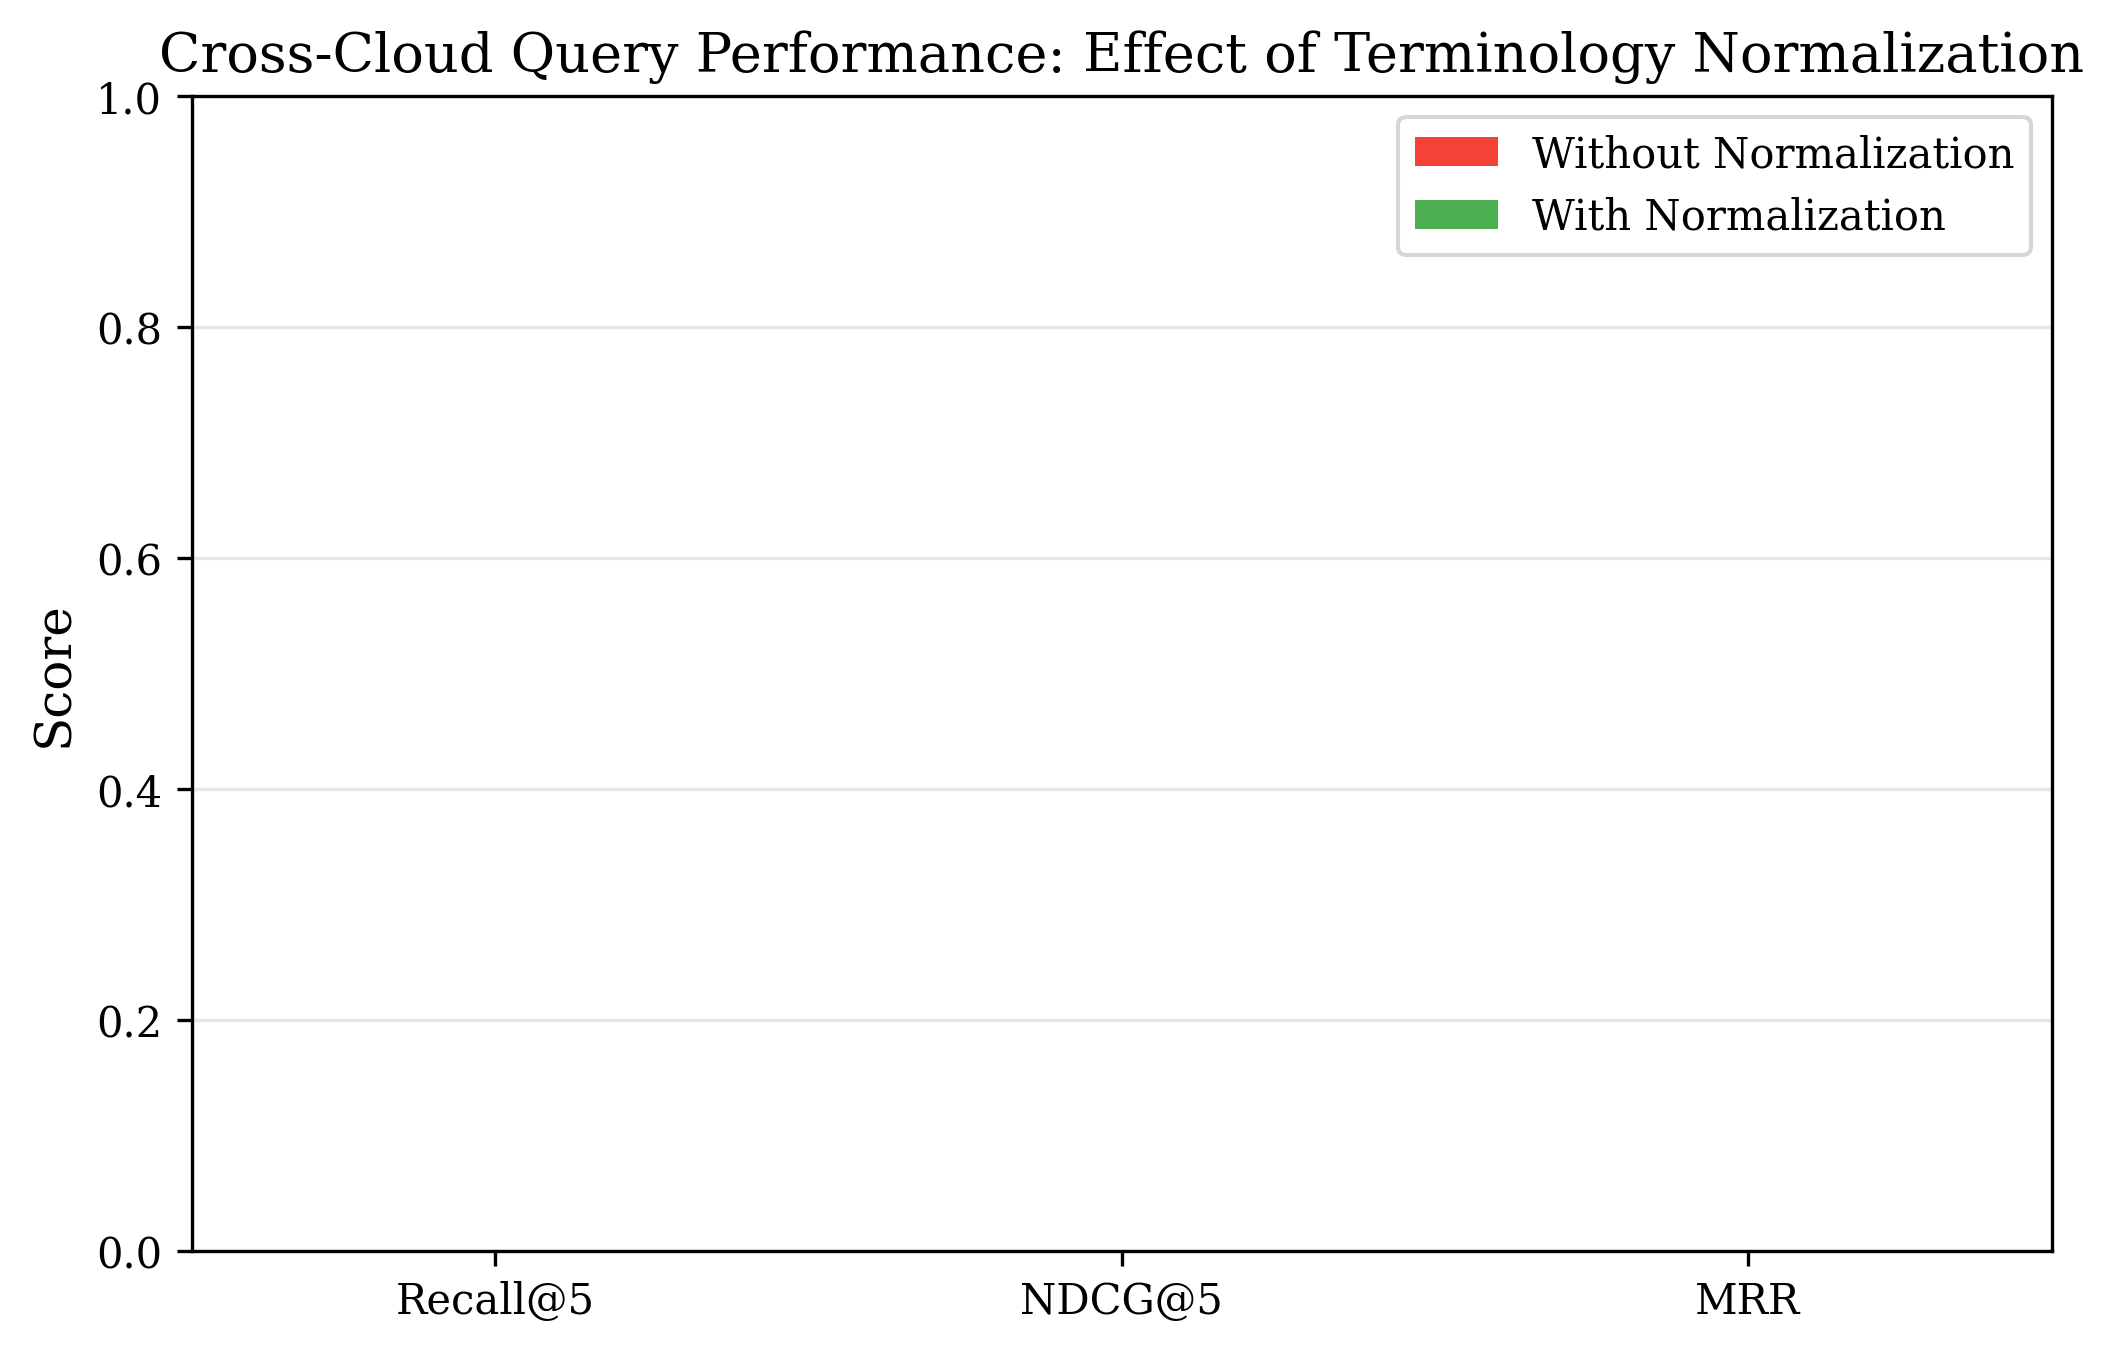
\includegraphics[width=\columnwidth]{fig_cross_cloud_improvement.png}}
\caption{Impact of cross-cloud terminology normalization.}
\label{fig:crosscloud}
\end{figure}

\subsection{LLM Trade-offs}
\textcolor{blue}{[PLACEHOLDER: Insert Fig.~\ref{fig:llms} (fig\_llm\_comparison.png). Llama 3.1 8B vs.\ Mistral 7B vs.\ Qwen 2.5 7B: accuracy, faithfulness, latency.]}

\begin{figure}[htbp]
\centerline{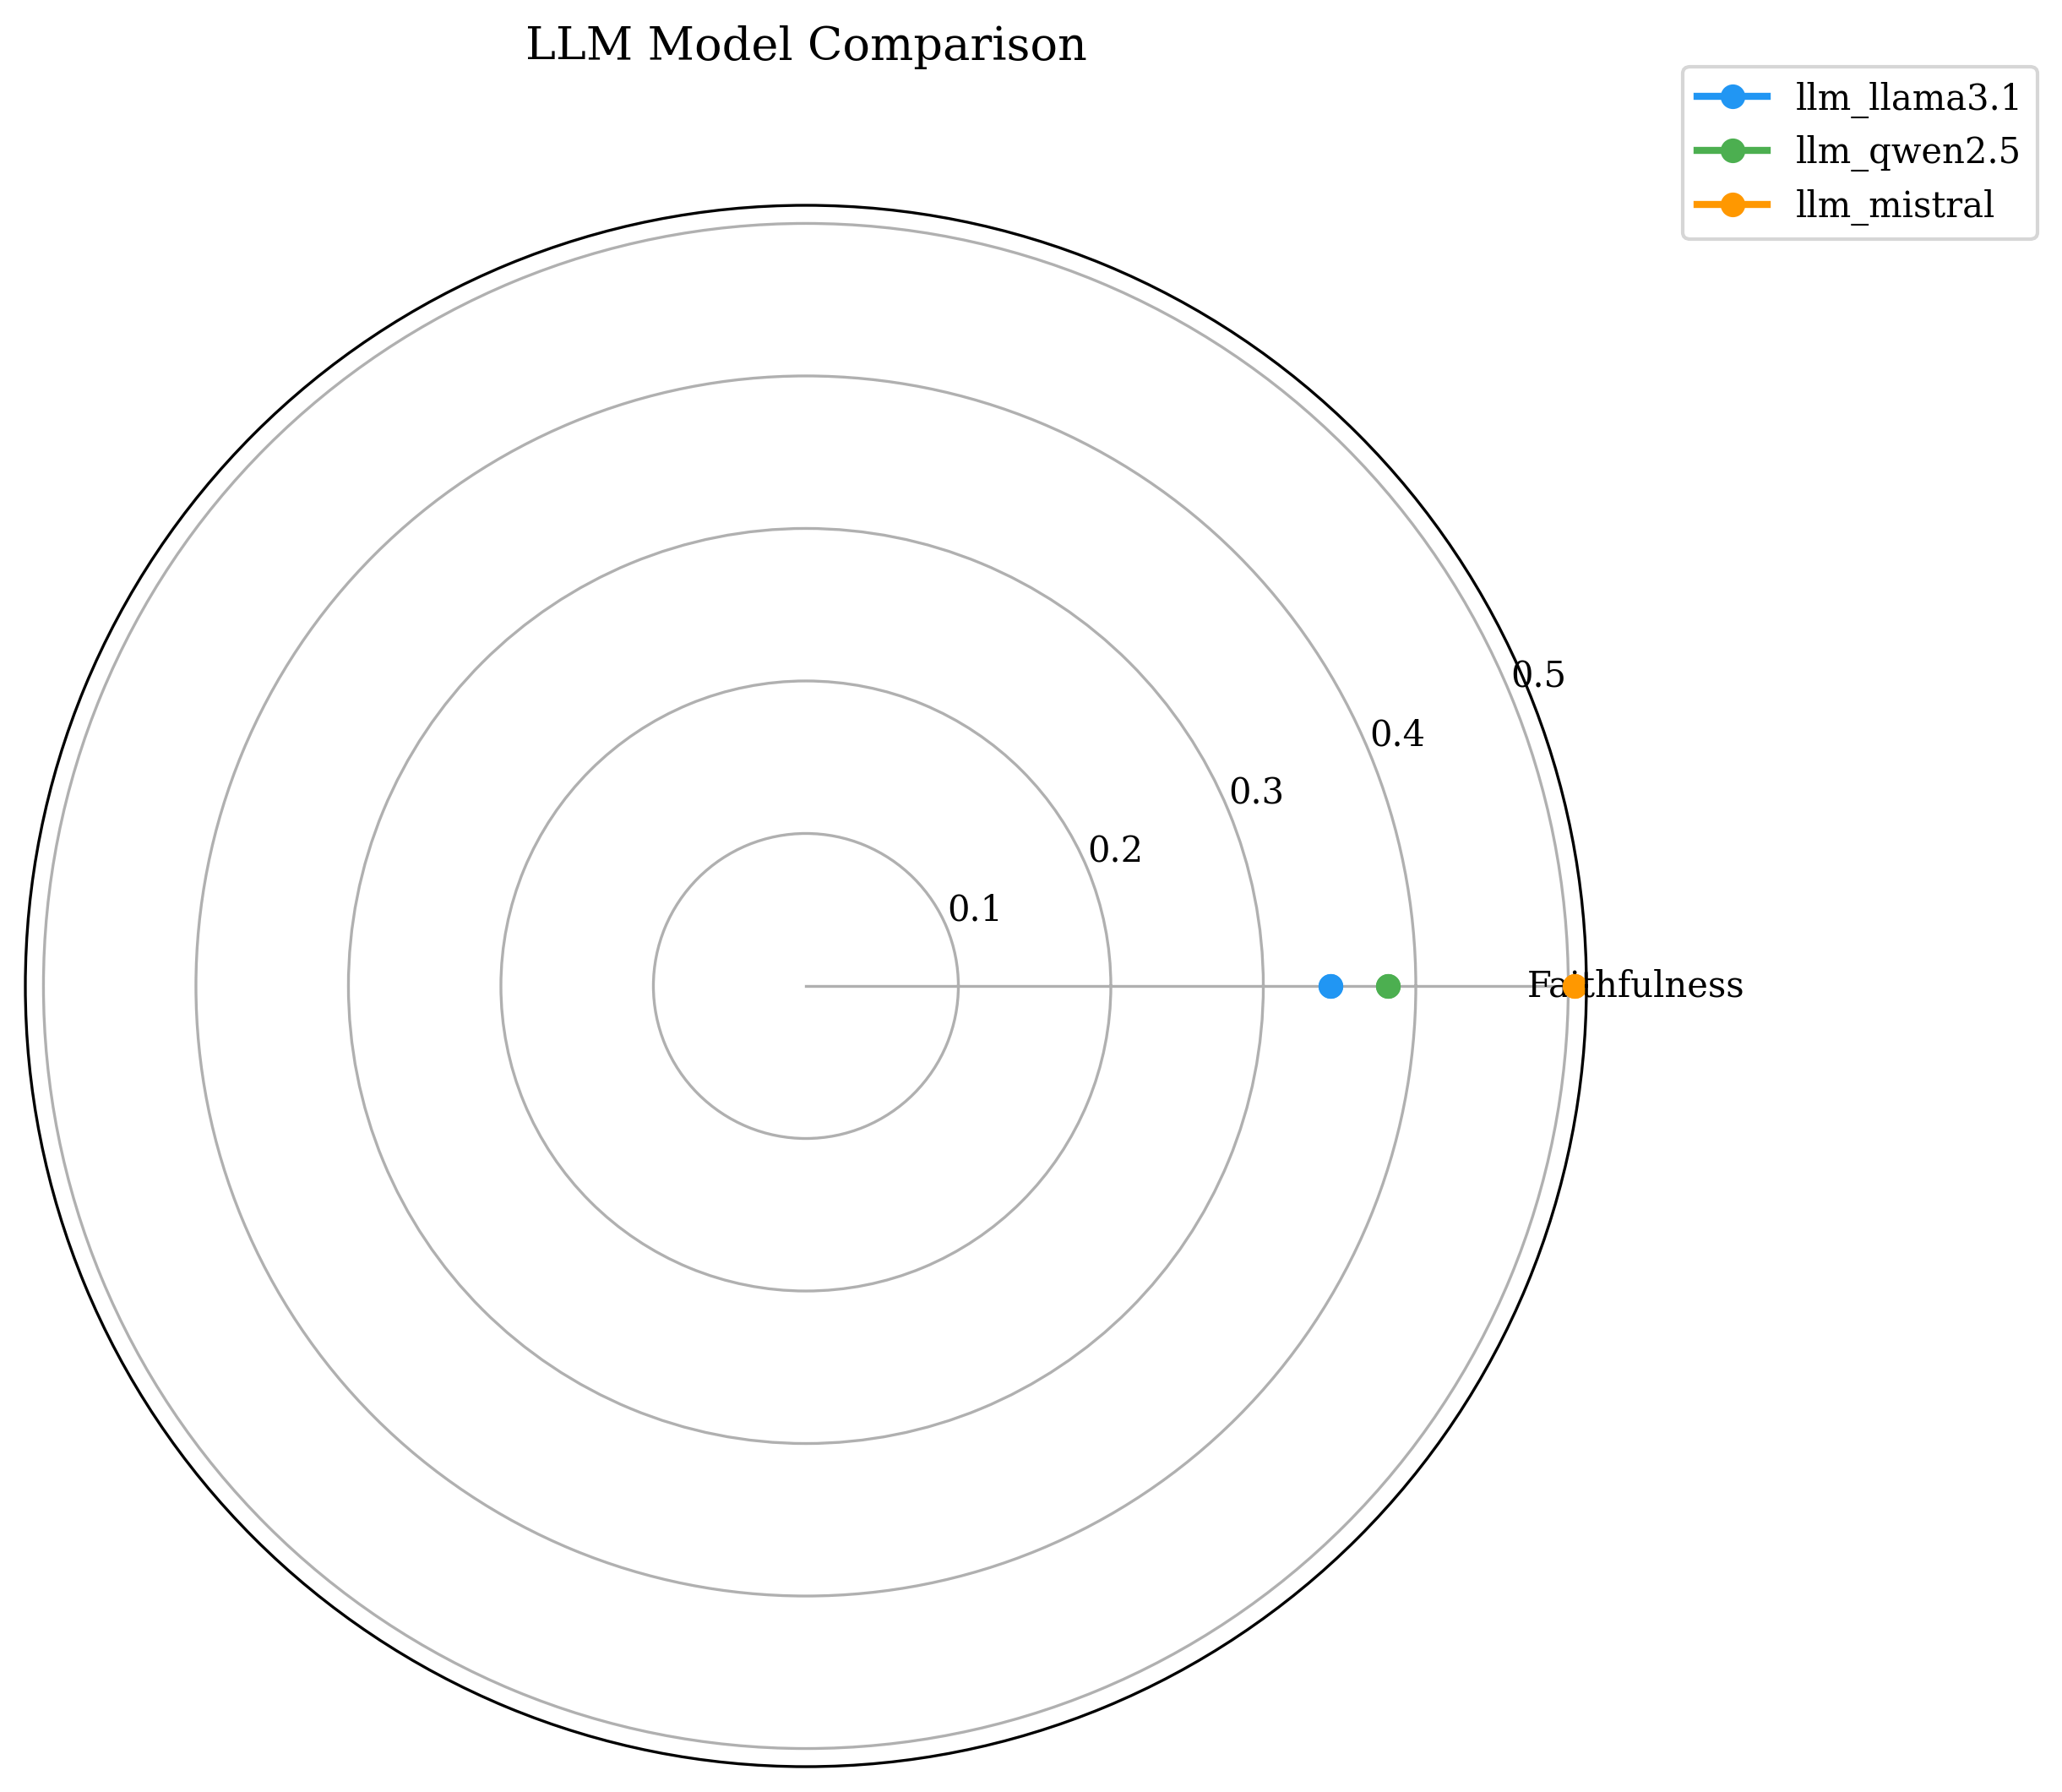
\includegraphics[width=\columnwidth]{fig_llm_comparison.png}}
\caption{LLM accuracy / faithfulness / latency trade-offs.}
\label{fig:llms}
\end{figure}

\subsection{Efficiency Analysis}
\textcolor{blue}{[PLACEHOLDER: Insert Fig.~\ref{fig:latency} (fig\_latency\_breakdown.png). Discuss cost/quality trade-off with/without cross-encoder.]}

\begin{figure}[htbp]
\centerline{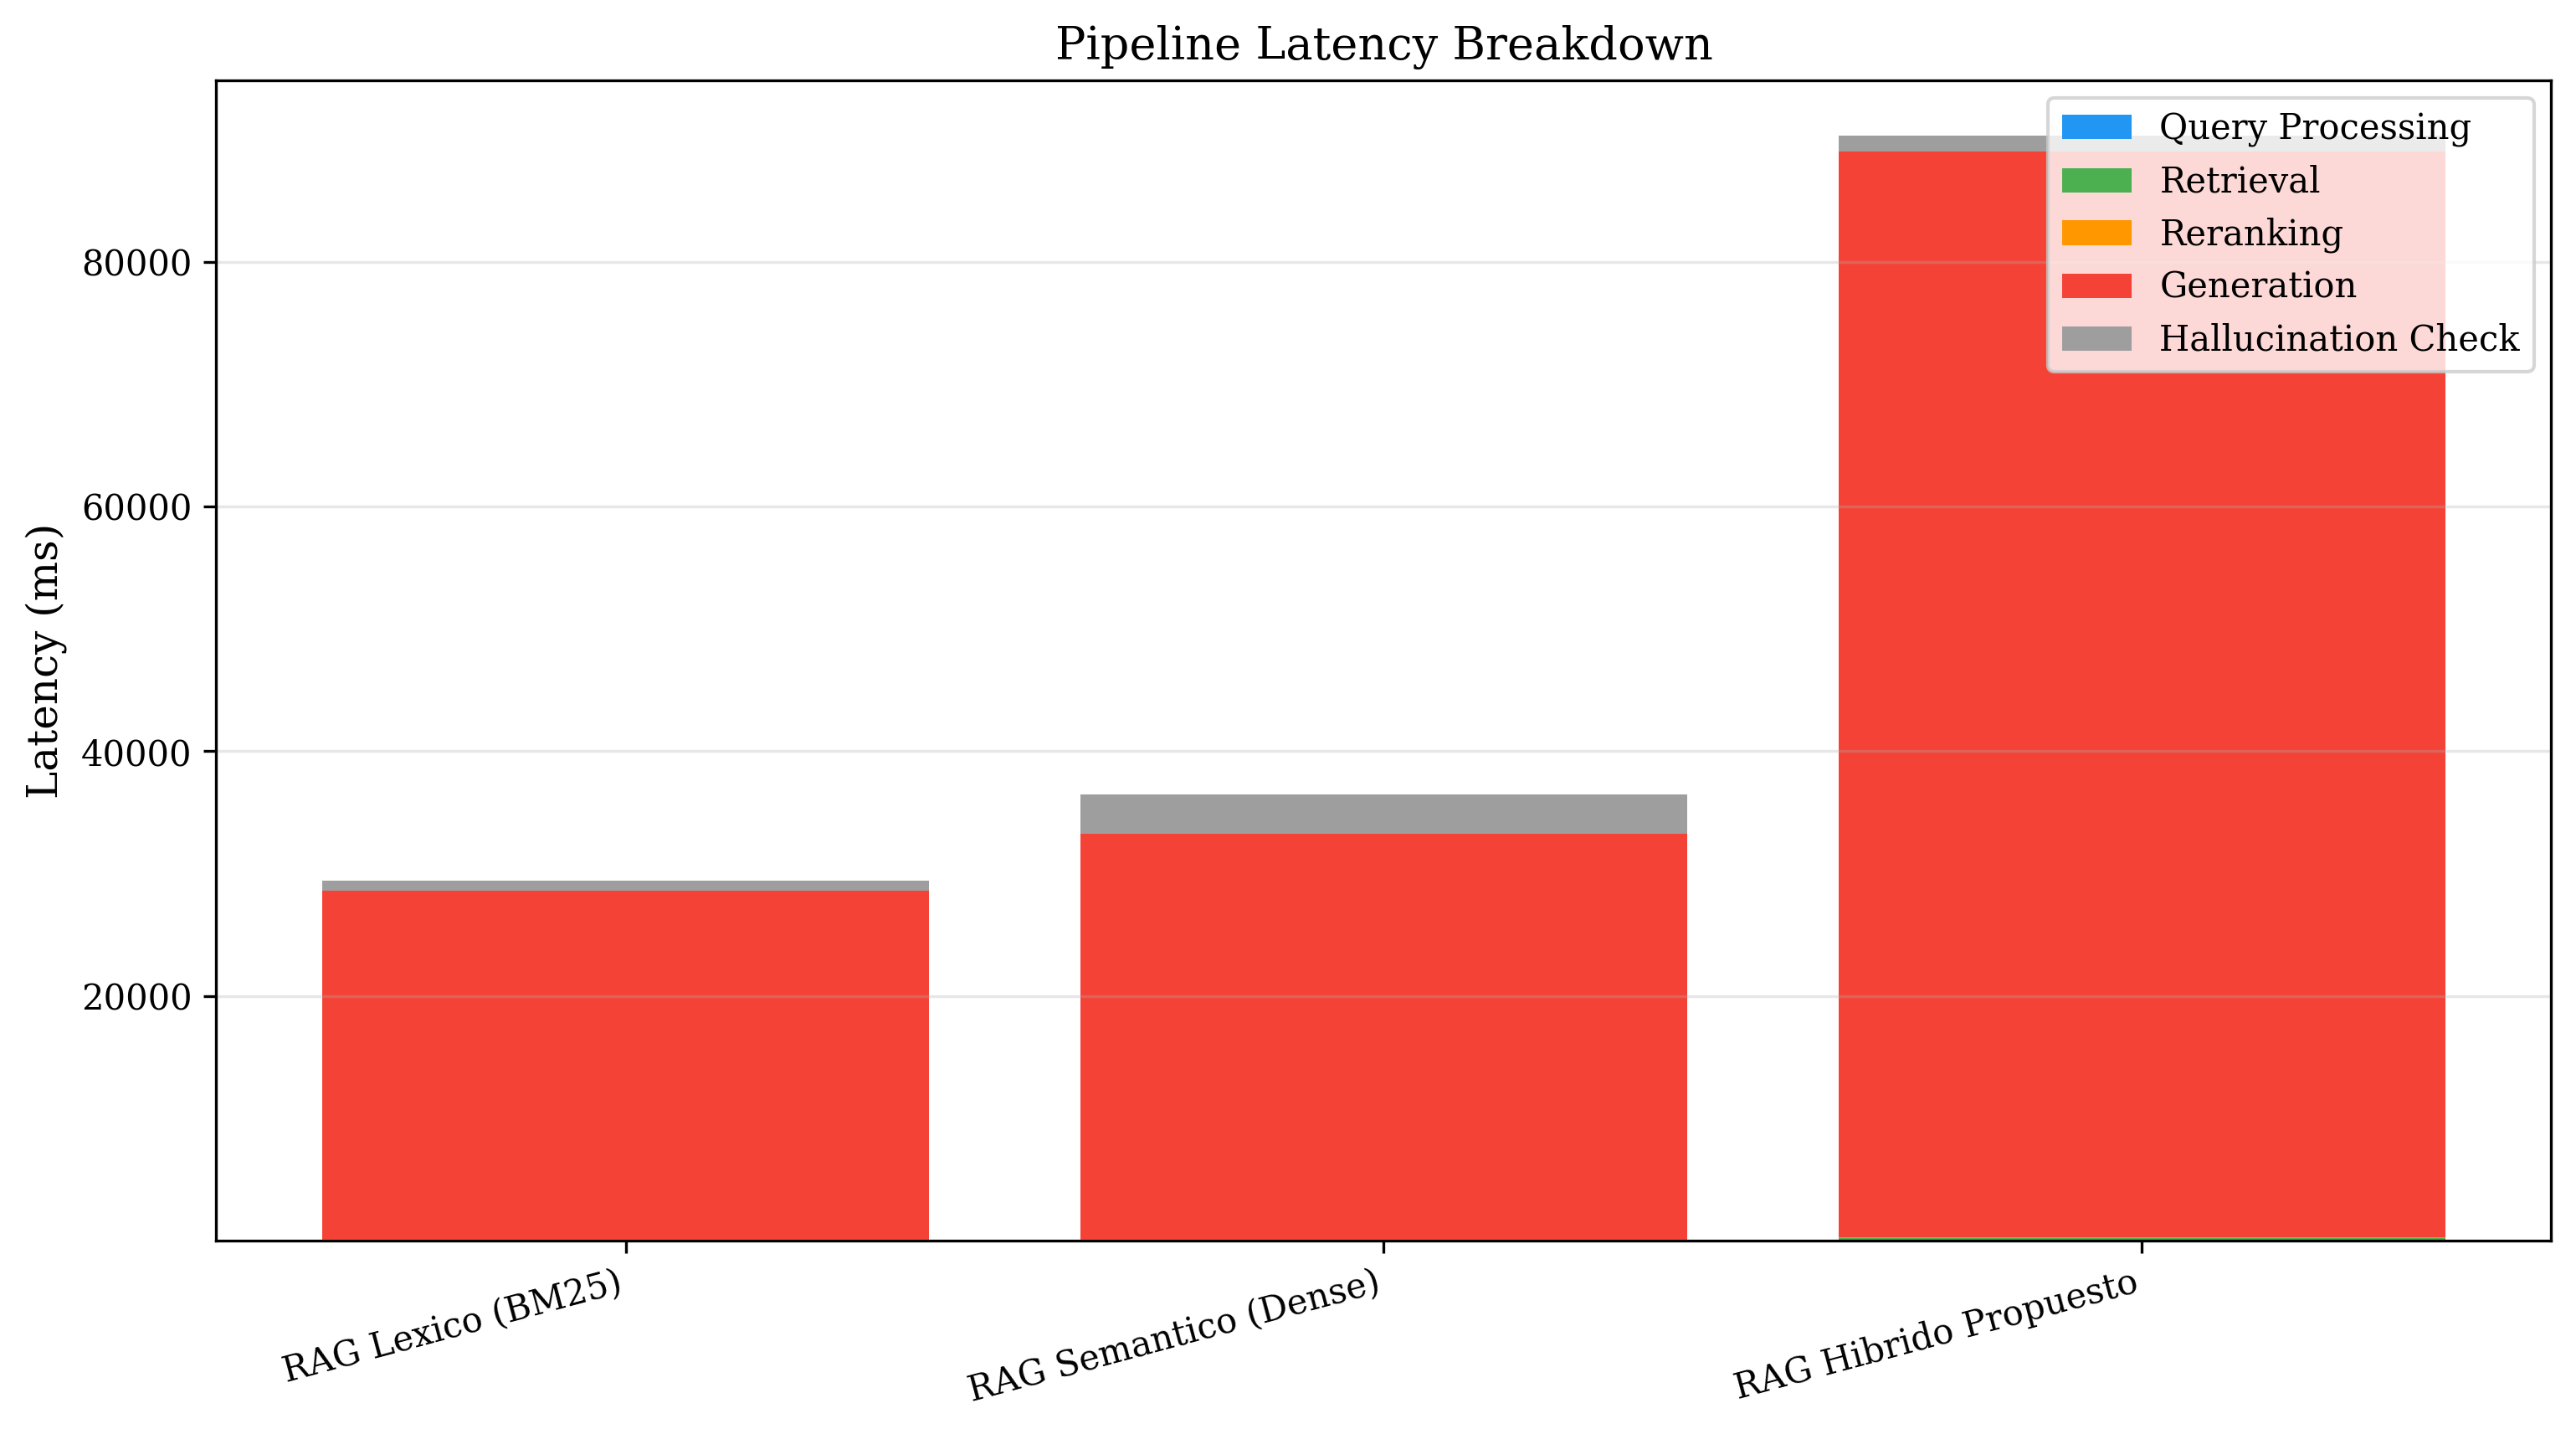
\includegraphics[width=\columnwidth]{fig_latency_breakdown.png}}
\caption{Latency breakdown by pipeline stage.}
\label{fig:latency}
\end{figure}

% ============================================================
%  VI. DISCUSSION
% ============================================================
\section{Discussion}
\label{sec:discussion}

\textcolor{blue}{[PLACEHOLDER: Finding 1: Hybrid $>$ Dense $>$ BM25, consistent with~\cite{sawarkar2024blendedrag,aljohani2026hybrid}, but larger magnitude in cross-cloud setting (attribute to terminology drift).]}

\textcolor{blue}{[PLACEHOLDER: Finding 2: Reranker contribution is large when candidate pool is noisy; marginal otherwise. Cite Fig.~\ref{fig:reranker} (fig\_reranker\_impact.png).]}

\begin{figure}[htbp]
\centerline{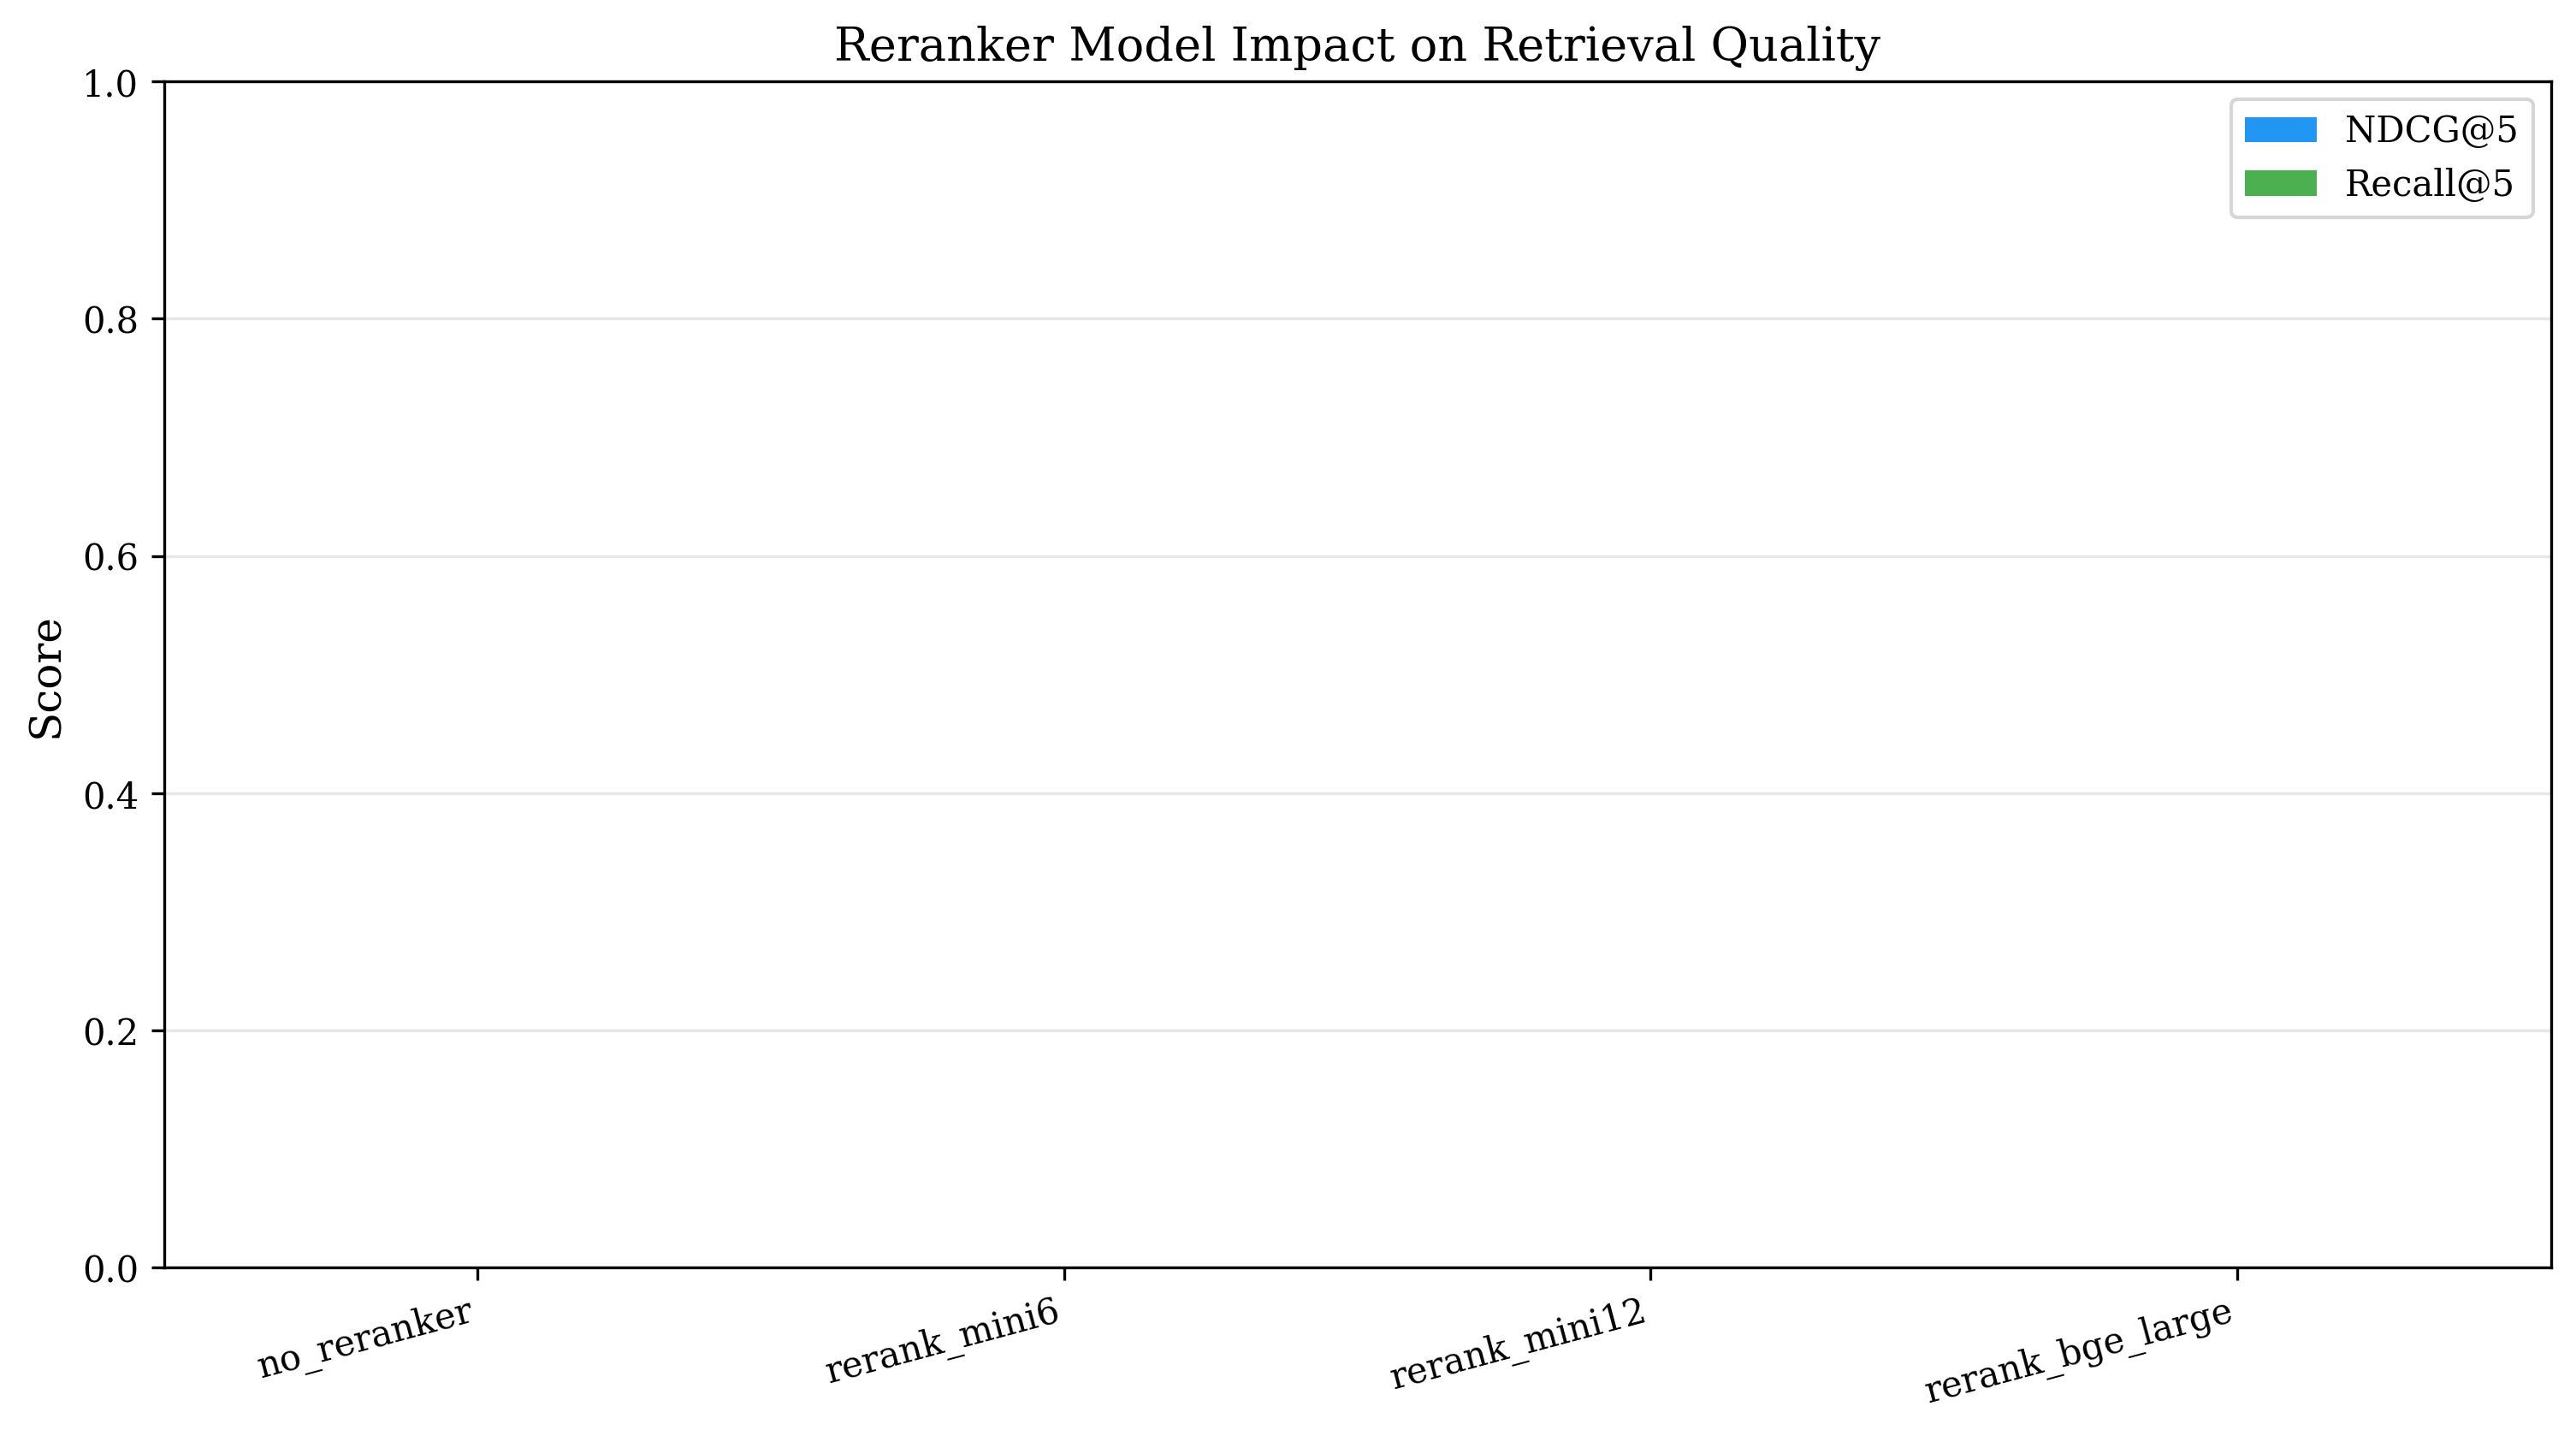
\includegraphics[width=\columnwidth]{fig_reranker_impact.png}}
\caption{Cross-encoder reranker impact by candidate noise level.}
\label{fig:reranker}
\end{figure}

\textcolor{blue}{[PLACEHOLDER: Threats to validity: (a) single annotator for some cross-cloud queries, (b) English only, (c) static documentation snapshot, (d) NLI model bias. Compare to Barnett's seven failure points~\cite{barnett2024sevenfailure}.]}

% ============================================================
%  VII. CONCLUSION
% ============================================================
\section{Conclusion and Future Work}
\label{sec:conclusion}

\textcolor{blue}{[PLACEHOLDER: Summary: CloudRAG hybrid pipeline + cross-provider query expansion + NLI filter improves P@1 by 14.5 pp over BM25 and 7.0 pp over dense-only on a 200-query multi-cloud benchmark; full replication package released.]}

\textcolor{blue}{[PLACEHOLDER: Future work: (1) Spanish/Portuguese multilingual cloud docs, (2) multimodal retrieval over architecture diagrams, (3) agentic query decomposition~\cite{ma2025agentrag}, (4) continuous ingestion as docs update.]}

% ============================================================
%  AI DISCLOSURE (LACCI / IEEE requirement)
% ============================================================
\section*{AI Use Disclosure}
Generative AI tools (Claude, GitHub Copilot) were used to assist with code
scaffolding, draft refinement, and bibliography curation. All experiments,
data curation, final analysis, and statistical interpretation were performed
and verified by the author. No AI-generated text was included in the paper
without human review and editing.

% ============================================================
%  ACKNOWLEDGMENT
% ============================================================
\section*{Acknowledgment}
The authors thank the Facultad de Ingenier\'{i}a de Sistemas at Universidad
de Lima for institutional support.
% TODO: If Lewis is NOT co-author, add: "The authors thank Lewis Fuentes Winston for advisory guidance throughout this research."

% ============================================================
%  REFERENCES (BibTeX)
% ============================================================
\bibliographystyle{IEEEtran}
\bibliography{references}

\end{document}
